%%
%% Arquivo principal para:
%% - teses de doutorado
%% - dissertaes de mestrado
%% - exames de qualificao de mestrado e doutorado
%%
%% NOTA: A PUBLICAO DESTE MODELO VISA APENAS ORIENTAR OS PS-GRADUANDOS
%% NA PREPARAO DE SEUS TEXTOS. O PPgEE DA UFRN NO PROV ASSISTNCIA NO
%% USO DAS FERRAMENTAS NECESSRIAS AO USO DESTE MODELO (LATEX, XFIG, ETC.)
%% 1
%% Adelardo Medeiros, dezembro de 2005.

% DEFINIES GLOBAIS

% Esta primeira linha d informaes gerais sobre o documento.
% PARA A VERSO FINAL:
% papel A4, letra grande (12pt), openr	sight (captulos s iniciam em
% pgina direita, se necessrio incluindo uma pgina em branco),
% twoside (o documento vai ser impresso em frente e costa)
%\documentclass[a4paper,12pt,openright,twoside]{book}
% PARA A QUALIFICAO E PARA A VERSO INICIAL:
% papel A4, letra grande (12pt), openany (captulos iniciam em
% qualquer pgina), oneside (o documento vai ser impresso s na frente)
\documentclass[a4paper,12pt,openany,oneside]{book}

% PACOTES OBRIGATRIOS
\usepackage{epigraph}
\usepackage{setspace}

%\usepackage{lipsum}
% Use estes pacotes para poder digitar diretamente as letras com acento
% e para que a hifenizao funcione corretamente
%\usepackage[latin1]{inputenc}
\usepackage[utf8]{inputenc}
\usepackage{ae}
% Para usar fontes standard ao invs das do LaTeX (gera melhores PDFs)
\usepackage{pslatex}
% Para a hifenizao em portugus
\usepackage[portuges, brazil]{babel}


% Para que os primeiros pargrafos das sees tambm sejam indentados
\usepackage{indentfirst}
% Para poder incluir grficos (figuras)
\usepackage{graphicx}
% Para poder fazer glossrio ou lista de smbolos
% Use a segunda opo se quiser incluir na definio do smbolo a
% pgina e/ou a equao onde ela foi definida
\usepackage[portuguese,noprefix]{nomencl}
%\usepackage[portuguese,noprefix,refeq,refpage]{nomencl}
% Para permitir espaamento simples, 1 1/2 e duplo
\usepackage{setspace}
% Para usar alguns comandos matemticos avanados muito teis
\usepackage{amsmath}
% Para poder usar o ambiente "comment"
\usepackage{verbatim}
% Para poder ter tabelas com colunas de largura auto-ajustvel
\usepackage{tabularx}
% Para executar um comando depois do fim da pgina corrente
\usepackage{afterpage}
% Para formatar URLs (endereos da Web)
\usepackage{url}
% Para reduzir os espaos entre os tens (itemize, enumerate, etc.)
% Este pacote no faz parte da distribuio padro do LaTeX.
\usepackage{noitemsep}
% Para as citaes bibliogrficas
\usepackage[abbr]{harvard}	% As chamadas so sempre abreviadas
\harvardparenthesis{square}	% Colchetes nas chamadas
%\harvardyearparenthesis{round}	% Parntesis nos anos das referncias
\renewcommand{\harvardand}{e}	% Substituir "&" por "e" nas referncias

% PACOTES OPCIONAIS

% Para poder incluir arquivos Postscript com cores (do Xfig, por exemplo)
\usepackage{color}
% Para ter clulas em tabelas que ocupam mais de uma linha
\usepackage{multirow}
\usepackage[table,xcdraw]{xcolor}
% Para poder ter tabelas longas em mais de uma pgina
%\usepackage{longtable}
% Para poder escrever partes do texto em "n" colunas
%\usepackage{multicol}
% Se voc quiser personalizar os cabealhos das pginas
%\usepackage{fancyheadings}
% Para incluir algoritmos e listagens de cdigos
\usepackage{listings}
% Captulos com ttulos em um formato "decorado"
\usepackage{capitulos}

\hyphenation{skinRGBDetect}

%FIGURAS LADO A LADO
\usepackage{subfigure}

% NOVOS COMANDOS

% As definies dos novos comandos esto agrupadas no arquivo "comandos.tex"
% Esta separao  opcional: se voc preferir, pode por as definies
% diretamente neste arquivo
% newcommand define novos comandos, que podem passar a ser usados da
% mesma forma que os comandos LaTeX de base.

% Implica��o em f�rmulas
\newcommand{\implica}{\quad\Rightarrow\quad} %Meio de linha
\newcommand{\implicafim}{\quad\Rightarrow}   %Fim de linha
\newcommand{\tende}{\rightarrow}
\newcommand{\BibTeX}{\textsc{B\hspace{-0.1em}i\hspace{-0.1em}b\hspace{-0.3em}}\TeX}

% Fra��o com parentesis
\newcommand{\pfrac}[2]{\left(\frac{#1}{#2}\right)}

% Transformada de Laplace e transformada Z
%\newcommand{\lapl}{\makebox[0cm][l]{\hspace{0.1em}\raisebox{0.25ex}{-}}\mathcal{L}}
\newcommand{\lapl}{\pounds}
\newcommand{\transfz}{\mathcal{Z}}

% N�o aparecer o n�mero na primeira p�gina dos cap�tulos
\newcommand{\mychapter}[1]{\chapter{#1}\thispagestyle{empty}}

% Os cap�tulos sem n�mero
\newcommand{\mychapterast}[1]{\chapter*{#1}\thispagestyle{empty}
\chaptermark{#1}
\afterpage{\markboth{\uppercase{#1}}{\rightmark}}
\markboth{\uppercase{#1}}{}
}

% Se��es sem n�mero
\newcommand{\mysectionast}[1]{\section*{#1}
\addcontentsline{toc}{section}{#1}
\markright{\uppercase{#1}}
}

% No tabularx, as celulas devem ser centradas verticalmente
\renewcommand{\tabularxcolumn}[1]{m{#1}}

% C�lulas centralizadas horizontalmente no tabularx
\newcolumntype{C}{>{\centering\arraybackslash}X}

%% Abrevia figuras e tabelas
%\def\figurename{Fig.}
%\def\tablename{Tab.}


%
% As margens
%

% Dire\c{c}\~{a}o horizontal

% Margem interna
% Nas pginas mpares
\setlength{\oddsidemargin}{3.5cm}         % Margem real desejada
% Nas pginas pares
\setlength{\evensidemargin}{2.5cm}        % Margem real desejada
% Largura do texto
\setlength{\textwidth}{15cm}
% As margens laterais no LaTeX so sempre 1 polegada maiores do que as
% fixadas. Se foi fixada \setlength{\oddsidemargin}{3.5cm}, a margem
% real seria de 3.5+2.54=6.04cm. Para permitir que voc no tenha que
% fazer esta conta, pode usar o nmero desejado nas linhas anteriores
% e a gente subtrai 1in nas prximas linhas
\addtolength{\oddsidemargin}{-1in}
\addtolength{\evensidemargin}{-1in}
% Note que a margem direita no  fixada diretamente:
% ela  obtida subtraindo-se os outros valores da largura da pgina.
% 3.5+15+x=21cm (largura A4) -> x = margem externa = 2.5cm

% Dire\c{c}\~{a}o vertical

% Margem superior (entre o topo da folha e o cabealho), altura do
% cabealho e distncia entre o fim do cabealho e o incio do texto
\setlength{\topmargin}{2.0cm}             % Margem real desejada
\setlength{\headheight}{1.0cm}
\setlength{\headsep}{1.0cm}
% Altura do texto (sem cabealho e rodap)
\setlength{\textheight}{22.7cm}
% Distncia do fim do texto ao rodap
\setlength{\footskip}{1.0cm}
% A margem superior no LaTeX  sempre 1 polegada maior do que a
% fixada. Se foi fixada \setlength{\topmargin}{2.0cm}, a margem
%real seria de 2.0+2.54=4.54cm. Para permitir que voc no tenha que
% fazer esta conta, pode usar o nmero desejado na linha anterior
% e a gente subtrai 1in na prxima linha
\addtolength{\topmargin}{-1in}
% Note que a margem inferior no  fixada diretamente:
% ela  obtida subtraindo-se os outros valores, sem incluir o
% "footskip", da altura da pgina.
% 2.0+1.0+1.0+22.7+x=29.7cm (altura A4) -> x = margem inferior = 3cm

%
% O estilo das referncias bibliogrficas
%

\bibliographystyle{ppgee}

%
% O espaamento entre linhas
%

% As pginas iniciais so sempre em espasamento simples
\singlespacing

% Para a criao do glossrio (ou lista de smbolos)
\makeglossary

% Lista de arquivos a serem processados. Estes comandos "includeonly" so
% dispensveis e devem obrigatoriamente ser comentados na hora de gerar o
% documento definitivo. Eles servem para compilar apenas parte do documento.
%  til, durante a redao, para que no se tenha de compilar todo o
% documento a cada vez que se faz uma alterao. Por exemplo, se eu estou
% fazendo alteraes na dedicatria e as outras partes no tm interesse no
% momento, posso incluir (descomentar) a linha "\includeonly{preambulo}"
%\includeonly{rosto}
%\includeonly{catalograficos}
%\includeonly{preambulo}
%\includeonly{resumos}
%\includeonly{capitulo1/introducao}
%\includeonly{capitulo2/metodologia}
%\includeonly{capitulo3/software}
%\includeonly{capitulo4/estudo}
%\includeonly{capitulo5/conclusao}
%\includeonly{apendice/apendice}

% ? inicio codigo fonte
\usepackage{listings}
\lstset
{
numbers=left,
stepnumber=5,
firstnumber=1,
numberstyle=\tiny,
extendedchars=true,
breaklines=true,
frame=tb,
basicstyle=\footnotesize,
stringstyle=\ttfamily,
showstringspaces=false
}
\renewcommand{\lstlistingname}{Listagem}
\renewcommand{\lstlistlistingname}{Lista de C\'{o}digos}
%=========================
% ? fim codigo fonte


% Inicia o texto
\begin{document}

% Paginas iniciais (sem numerao)
\pagestyle{empty}

% P\'{a}gina de rosto (capa interna)
%
% ********** Pagina de Rosto
%

% titlepage gera paginas sem numera\c{c}ao
\begin{titlepage}

\begin{center}

\small

% O comando @{} no ambiente tabular x  para criar um novo delimitador
% entre colunas que no a barra vertical | que  normalmente utilizada.
% O delimitador desejado vai entre as chaves. No exemplo, no h nada,
% de modo que o delimitador  vazio. Este recurso est sendo usado para
% eliminar o espao que geralmente existe entre as colunas
\begin{tabularx}{\linewidth}{@{}l@{}C@{}r@{}}
% A figura foi colocada dentro de um parbox para que fique verticalmente
% centralizada em relao ao resto da linha
\parbox[c]{3cm}{
\includegraphics[width=\linewidth]{LogoUFRN}} &
\begin{center}
\textsf{\textsc{Universidade Federal do Rio Grande do Norte\\
Centro de Tecnologia\\
Departamento de Engenharia de Computa\c{c}\~{a}o e Automa\c{c}\~{a}o\\
Curso de Engenharia de Computa\c{c}\~{a}o}}
\end{center}
\end{tabularx}


% O vfill  um espao vertical que assume a mxima dimenso possvel
% Os vfill's desta pgina foram utilizados para que o texto ocupe
% toda a folha
\vfill

\LARGE

\textbf{ANÁLISE DA VIABILIDADE DO USO DE XBEE PARA A IMPLEMENTAÇÃO DE UMA REDE MULTI VANTS}

\vfill

\Large

\textbf{Filipe Viana Monteiro}

\vfill
%
\normalsize

Orientador: Prof. Dr. Pablo Javier Alsina
% Se no houver co-orientador, comente a pr\'{o}xima linha
%\\[2ex] Co-orientador: Prof. Dr. Beltrano Catandura do Amaral

\vfill



%\textbf{Disserta\c{c}\~{a}o de Mestrado}
%\textbf{Tese de Doutorado}
%apresentada ao Programa de P\'{o}s-Gradu\c{c}\~{a}o em Engenharia El\'{e}trica da UFRN
%(\'{a}rea de concentra\c{c}\~{a}o: Automa\c{c}\~{a}o e Sistemas)
%(\'{a}rea de concentra\c{c}\~{a}o: Telecomunica\c{c}\~{o}es)
%como parte dos requisitos para obten\c{c}\~{a}o do t\'{\i}tulo de
%Mestre em Ci\^{e}ncias.}
%Doutor em Ci\^{e}ncias.}

\vfill

\large

Natal/RN

Dezembro de 2016

\end{center}

\end{titlepage}



% Ficha catalografica: os dados catalogrficos devem ser fornecidos
% pela BCZM.
% S\'{o} s\~{a}o inclu\'{\i}dos na vers\~{a}o final da tese ou disserta\c{c}\~{a}o. N\~{a}o s\~{a}o
% inclu\'{\i}dos nem na proposta de tema de qualificao nem na vers\~{a}o
% preliminar da tese ou disserta\c{c}\~{a}o: nestes casos, comente a pr\'{o}xima linha.

%%
% ********** Ficha Catalogr�fica
%

\newpage

\begin{center}

% Aqui n�o se usou \vfill porque o \vfill � constru�do internamente com
% o comando \vspace. Espa�os verticais no in�cio da folha com \vspace
% s�o ignorados. Para que isto n�o ocorra deve-se usar o \vspace*
% \vspace*{\fill} � como se fosse um \vfill*
\vspace*{\fill}

Divis�o de Servi�os T�cnicos\\[1ex]
Cataloga��o da publica��o na fonte.
UFRN / Biblioteca Central Zila Mamede

\vspace{2ex}

\begin{tabular}{|p{0.9\linewidth}|} \hline
\\
Pereira, Fulano dos Anz�is.\\
\hspace{1em} Sobre a Prepara��o de Propostas de Tema, Disserta��es
e Teses no Programa de P�s-Gradua��o em Engenharia El�trica da UFRN /
Fulano dos Anz�is Pereira - Natal, RN, 2006 \\
\hspace{1em} 23 p. \\
\\
\hspace{1em} Orientador: Sicrano Matosinho de Melo \\
\hspace{1em} Co-orientador: Beltrano Catandura do Amaral \\
\\
\hspace{1em} Tese (doutorado) - Universidade Federal do Rio Grande do Norte.
Centro de Tecnologia. Programa de P�s-Gradua��o em Engenharia El�trica. \\
\\
\hspace{1em} 1. Reda��o t�cnica - Tese. 2. \LaTeX - Tese.
I. Melo, Sicrano Matosinho de. II. Amaral, Beltrano Catandura do.
III. T�tulo. \\
\\
RN/UF/BCZM \hfill CDU 004.932(043.2) \\ \hline
\end{tabular} 

\end{center}


% Assinaturas da banca, dedicatria e agradecimentos
% S\'{o} s\~{a}o inclu\'{\i}dos na verso final da tese ou dissertao. N\~{a}o s\~{a}o
% inclu\'{\i}dos nem na proposta de tema de qualifica\c{c}\~{a}o nem na vers\~{a}o
% preliminar da tese ou dissertao: nestes casos, comente a pr\'{o}xima linha.
% ********** P\'{a}gina de assinaturas
%

\begin{titlepage}
%
\begin{center}
%

%
\Large \textbf{Análise da Viabilidade do Uso de Xbee para a Implementação de um Rede Multi VANTs}


\vfill

\Large \textbf{Filipe Viana Monteiro}

\bigskip
\bigskip
\bigskip
\bigskip

\normalsize

Orientador: Prof. Dr. Pablo Javier Alsina

\vfill

\hfill
\parbox{0.5\linewidth}{
% Descomente as opes que se aplicam ao seu caso
\textbf{Monografia}
apresentada \`{a} Banca Examinadora do Trabalho de Conclus\~{a}o do Curso de
Engenharia de Computa\c{c}\~{a}o, em cumprimento \`{a}s exig\^{e}ncias
legais como requisito parcial \`{a} obten\c{c}\~{a}o do t\'{\i}tulo de Engenheiro de
Computa\c{c}\~{a}o.}

\vfill

\large

Natal/RN

Dezembro de 2016

\end{center}
\end{titlepage}

%
% ********** Dedicat\'{o}ria
%

% A dedicat\'{o}ria n\~{a}o \'{e} obrigat\'{o}ria. Se voc\^{e} tem algu\'{e}m ou algo que teve
% uma import\^{a}ncia fundamental ao longo do seu curso, pode dedicar a ele(a)
% este trabalho. Geralmente n\~{a}o se faz dedicat\'{o}ria a v\'{a}rias pessoas: para
% isso existe a se\c{c}\~{a}o de agradecimentos.
% Se n\~{a}o quiser dedicat\'{o}ria, basta excluir o texto entre
% \begin{titlepage} e \end{titlepage}

\begin{titlepage}

\vspace*{\fill}

\hfill
\begin{minipage}{0.5\linewidth}
\begin{flushright}
\large\it
Aos meus pais, Américo Monteiro Filho e Rosalba Viana Monteiro, que com todos os esforços, puderam me proporcionar a melhor educação possível.

\end{flushright}
\end{minipage}

\vspace*{\fill}

\end{titlepage}

%
% ********** Agradecimentos
%

% Os agradecimentos n\~{a}o s\~{a}o obrigat\'{o}rios. Se existem pessoas que lhe
% ajudaram ao longo do seu curso, pode incluir um agradecimento.
% Se n\~{a}o quiser agradecimentos, basta excluir o texto ap\'{o}s \chapter*{...}

\chapter*{Agradecimentos}
\thispagestyle{empty}

\begin{trivlist}  \itemsep 2ex

\item Primeiramente tenho que agradecer ao meus pais, Américo Monteiro Filho e Rosalba Viana Monteiro, que sempre me possibilitaram o melhor ensino que nos era acessível. Nunca esquecerei o esforço que fizeram, e ainda fazem, para educar a mim e a minha irmã Andreza. Espero um dia poder me torna um pai tão bom quanto vocês.
  
\item Também devo agradecer aos amigos que sempre me apoiaram durante minha trajetória académica, seja ajudando a entender os conteúdos de sala de aula ou me ajudando a esquecer um pouco desses conteúdos e aliviar um pouco minha cabeça de toda a pressão que é a vida universitária.

\item Por fim tenho que agradecer, em especial, a excepcional turma de Engenharia da Computação formada em 2013, a qual faço parte. Acho que a nossa união foi um ponto que ajudou bastante na nossa formação. Nunca esquecerei das noites de estudos e projetos no DCA. E que venham muitas terças da pizza naquele mesmo lugar para comemorar nossas conquistas daqui pra frente.

\item Muito Obrigado a todos vocês.

\end{trivlist}

%\newpage

%\vspace*{\fill}
%\setlength{\epigraphrule}{1pt}
%\onehalfspacing
%\setlength{\epigraphwidth}{.95\textwidth}

%\begin{epigraphs}
%\qitem{
%    \textit{
%        \linebreak "Já dizia Tobias"
%        }
%    }
%{\textsc{Autor Desconhecido}}
%\end{epigraphs}



%\vspace*{\fill}


%
% O espa\c{c}amento entre linhas
%

% PARA A VERS\~{A}O FINAL:
% Deve ser usado espa\c{c}amento simples nas p\'{a}ginas de texto
%\singlespacing
% PARA A QUALIFICA\c{C}\~{A}O E PARA A VERS\~{A}O INICIAL:
% Deve ser usado espa\c{c}amento 1 1/2 nas pginas de texto
\onehalfspacing

% Resumo/Abstract
%% Resumo %%

\mychapterast{Resumo}

Este trabalho apresenta o desenvolvimento e explicação detalhada de uma aplicação que integra elementos de sistemas industriais (sensores, controladores e transmissores, por exemplo) com sistemas supervisórios, tornando possível a obtenção de dados desses elementos e controle das grandezas por eles medidas. O trabalho foi realizado com base em uma planta industrial que simula sistemas petrolíferos, presente no Laboratório de Avaliação de Medição em Petróleo (LAMP), que comporta elementos de instrumentação que necessitam serem lidos e manipulados através de Controladores Lógicos Programáveis (CLPs) e Sistemas de Supervisão e Aquisição de Dados (SCADA). O projeto realizado resume-se em captar os dados de sensores presentes nesse sistema industrial através de um CLP e um microcontrolador e realizar a comunicação destes com uma aplicação de supervisão desenvolvida no software Elipse SCADA. Foram utilizados CLPs da fabricante WEG modelo TPW03 e um microcontrolador da NOVUS modelo N2000. A comunicação foi realizada utilizando protocolo Modbus.



\textbf{Palavras-chave}: CLP; SCADA; Comunicação; TPW03; N2000; Modbus.

\mychapterast{Abstract}

This work presents the development and detailed explanation of an application that integrates elements of industrial systems (sensors, controllers and transmitters, for example) with supervisory systems, making it possible to obtain data of these elements and control the quantities they measures. The work was carried out on an industrial plant that simulates petroleum systems present in the Laboratório de Avaliação de Medição em Petróleo (LAMP), which includes instrumentation elements that need to be read and handled by programmable logic controllers (PLCs) and a Supervisory Control and Data Acquisition (SCADA) system. The project can be summarized by capturing data from sensors present in this industrial system through a PLC and a microcontroller and perform communication of these elements with a supervision application developed on Elipse SCADA software. We used WEG's PLC TPW03 and a NOVUS' microcontroller N2000 model. The communication was performed using Modbus protocol.


\textbf{Keywords}: PLC; SCADA; Communication; TPW03; N2000; Modbus.

% P\'{a}ginas introdut\'{o}rias (com numera\c{c}\~{a}o romana)
\frontmatter

% Lista de conte\'{u}do (gerado automaticamente)
\addcontentsline{toc}{chapter}{Sum\'{a}rio}
\tableofcontents

%%% Lista de figuras (gerada automaticamente)
\cleardoublepage
\addcontentsline{toc}{chapter}{Lista de Figuras}
\listoffigures

% Lista de tabelas (gerada automaticamente)
%\cleardoublepage
%\addcontentsline{toc}{chapter}{Lista de Tabelas}
%\listoftables

% Gloss\'{a}rio (gerado automaticamente - veja entradas em
% introducao/introducao.tex e em estilo/estilo.tex)

%\cleardoublepage
%\renewcommand{\nomname}{Lista de S\'{\i}mbolos e Abreviaturas}
%\markboth{\MakeUppercase{\nomname}}{\MakeUppercase{\nomname}}
%\addcontentsline{toc}{chapter}{\nomname}

% O argumento opcional do comando \printglossary  a largura deixada
% para os s\'{\i}mbolos no gloss\'{a}rio. Se seus s\'{\i}mbolos s\~{a}o "largos", como
% neste exemplo, \'{e} melhor por mais espa\c{c}o do que o 1cm que  reservado
% por default
%printglossary{1.5cm}% P\'{a}ginas do texto principal (com cabealho)
\mainmatter
\pagestyle{headings}

% Para facilitar a organiza\c{c}\~{a}o, foi criado um diretorio para cada
% captulo do documento, pois assim os arquivos das figuras ficam
% classificados por captulos

% Gerar Refer\^{e}ncias - bibtex principal
% Gerar Gloss\'{a}rio - makeindex -s nomencl.ist -o principal.gls principal.glo

% Comente Introduo abaixo e descomente seu capitulo

\mychapter{Introdução}
\label{Cap:introducao}

A utilização de veículos não tripulados já é bastante evidente em aplicações tanto civis quanto militares. Podem-se encontrar veículos dessa categoria substituindo a presença humana em situações onde há risco a integridade física ou quando o acesso é simplesmente impossível. Dentre os veículos não tripulados, temos a categoria de veículos aéreos não tripulados (VANTs) que são usados largamente para realização de filmagens aérea a baixo custo. Com o investimento de algumas centenas de dólares, qualquer pessoa pode começar a produzir imagens aéreas utilizando VANTs comerciais. O mercado está repleto de modelos comerciais disponíveis para o público em geral, como por exemplo os quadrirrotores fabricados pela DJI, o recém anunciado Karma fabricado pela GoPro, entre outros.

Como citado anteriormente, as aplicações para veículos aéreos não tripulados não se restringe ao uso civil ou para gravação de imagens aéreas, esta plataforma já vem sendo utilizada também em aplicações militares. Ao aliar o poder da plataforma em questão com outras tecnologias, como por exemplo o processamento digital de imagens, problemas mais complexos podem ser resolvidos. 

Um problema que pode ser solucionado com a utilização de VANTs dotados de ferramentas para processamento digital de imagem seria a identificação de embarcações não autorizadas em área de impacto de foguetes, problema esse relevante ao Centro de Lançamento Barreira do Inferno (CLBI) localizada em Natal no Rio Grande do Norte. 

Em parceria com a Universidade Federal do Rio Grande do Norte (UFRN), através do projeto de pesquisa SPACEVANT coordenado pelo professor Dr. Pablo Javier Alsina, o CBLI vem desenvolvendo uma solução, incluindo software e hardware, para a realização da verificação da aérea de impacto de foguetes de forma autônoma utilizando VANTs. 

\section{Objetivos}

Como parte do desenvolvimento dessa solução, esse trabalho tem por objetivo validar as especificações técnicas do transmissor XBEE PRO S3 900HP adquirido para a implementação da rede de comunicação e a viabilidade da utilização desse tipo de equipamento no contexto de uma rede multi VANT.

A fim de realizar essa validação, foram realizados teste de força de sinal e taxa de transferência de pacotes em uma rede mesh/ad hoc, implementada por módulos XBee PRO S3 900HP, usando quadrirrotores Phantom 3 do modelo Standard fabricados pela DJI para variar a distância entre os pontos da rede e, posteriormente, verificar os efeitos do distanciamento nos parâmetros estudados.

\section{Estrutura do Trabalho}

Após este capitulo introdutório, é apresentada uma breve descrição do projeto SpaceVANT a fim de familiarizar o leitor com o contexto desse trabalho. Em seguida, no capítulo 3, são discutidos os requisitos aos quais uma rede multi VANTs deve atender. 

A estratégia de varredura de area desenvolvida pelo mestrando Maurício Rabello para o projeto é apresentada no capítulo 4. Em seguida, o procedimento experimental desenvolvido, bem como os equipamentos utilizados para a sua realização, são apresentados no capítulo 5.

Por fim temos a discussão dos resultados experimentais e a conclusão do trabalho nos capítulos 6 e 7, respectivamente.  

\mychapter{Esrtutura do Sistema}
\label{Cap:estruturaSistema}




\mychapter{Implementações}
\label{Cap:implementacoes}



\mychapter{Aplicação e Testes}
\label{Cap:aplicacaoTestes}

\section{Desenvolvimento do Sistema Supervisório}

O sistema supervisório é desenvlvido através de uma aplicação no Elipse SCADA. A finalidade desse sistema é a seguinte: através da comunicação Modbus, deve se feita com sucesso a leitura de dois sensores de temperatura, sendo um deles ligado ao módulo analógico do TPW-03 e o outro ao N2000 e demonstrar graficamente a variação dos valores descritos por eles quando submetidos à mudanças de temperatura. 

Tendo em vista o objetivo do sistema, cria-se em uma tela, dois objetos do tipo '\textit{Guage}' que irá indicar o valor de temperatura apontado pelos sensores, um '\textit{Trend Graph}' que plota a temperatura descrita nos sensores a cada 0.5 segundos e um '\textit{Bar Graph}' que torna mais clara a observação da diferença de temperatura que cada sensor está medindo em determinado instante de tempo. A interface desenvolvida é observada na Figura \ref{fig:Interface}.

\begin{figure}[h!]
\centering
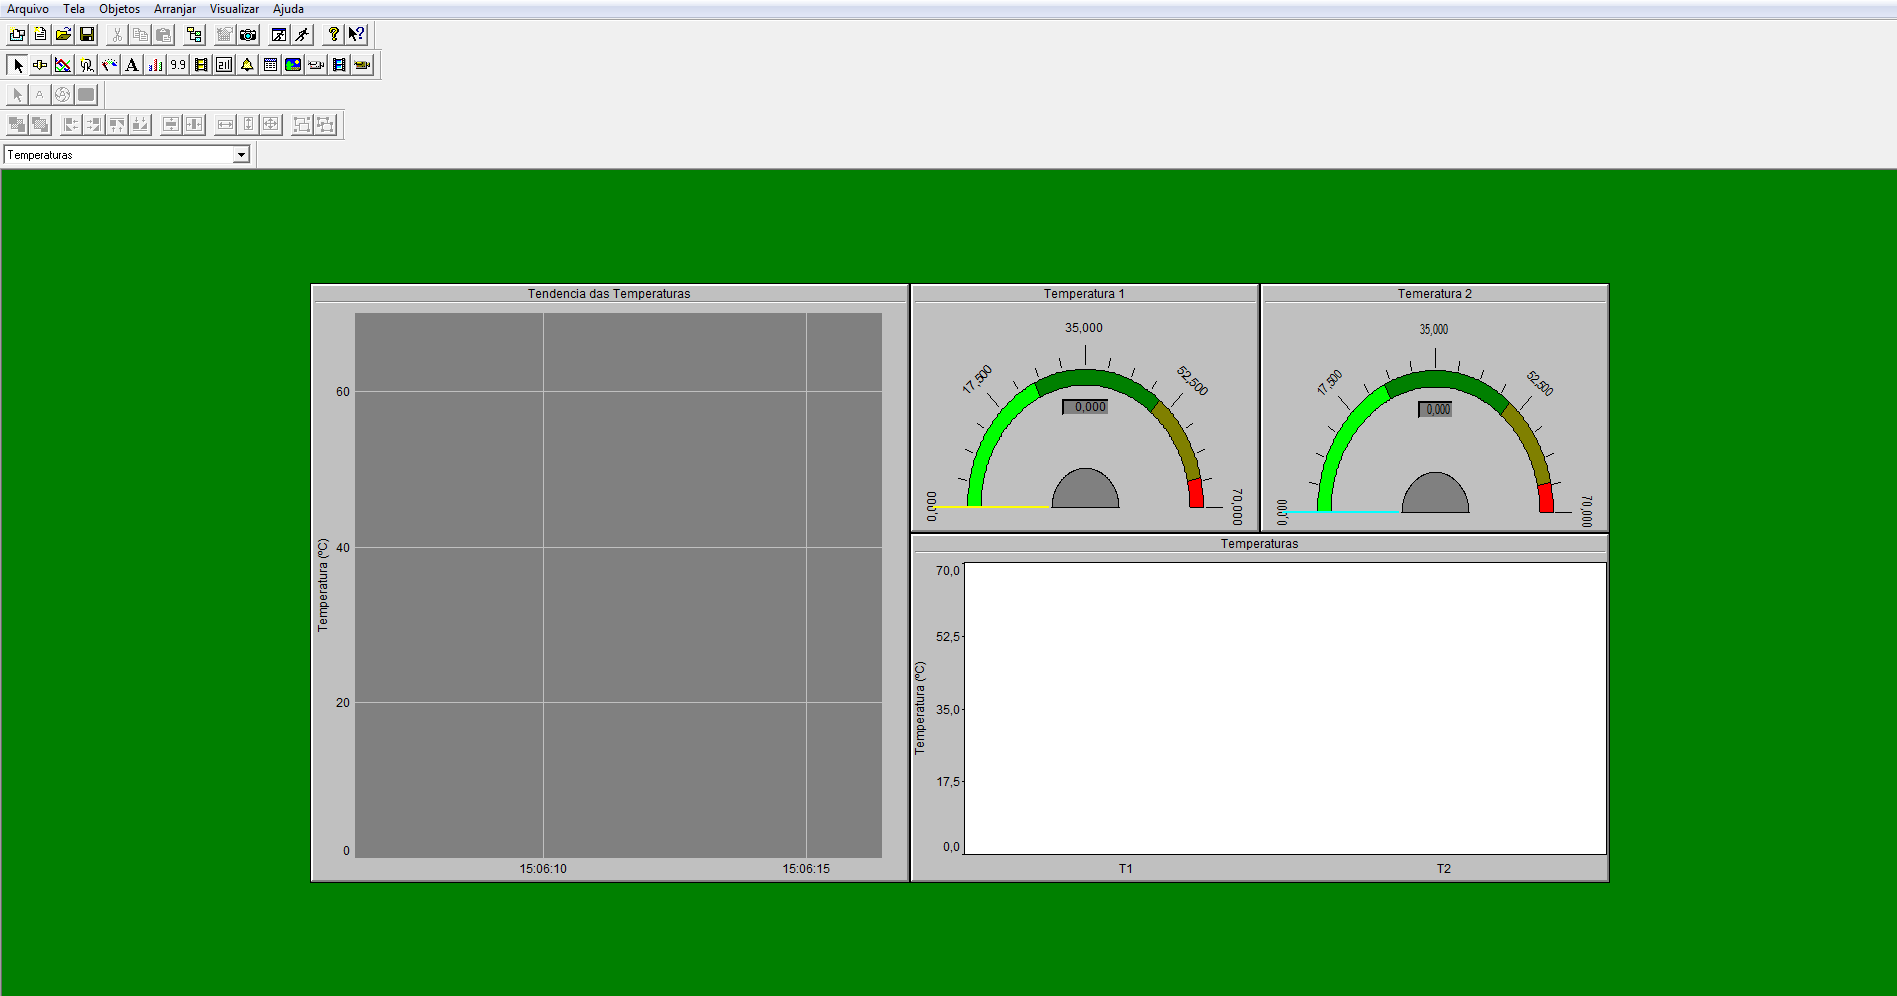
\includegraphics[scale=0.29]{Interface.png}
\caption{Interface da Aplicação}
\label{fig:Interface}
\end{figure}

Utilizando a ferramenta \textit{Organizer} do Elipse SCADA, criam-se duas \textit{tags} do tipo PLC, as quais irão armazenar as variáveis que indicam os valores das temperaturas fornecidas pelos sensores. Como essa aplicação consiste em um teste de conexão e leitura de apenas dois sensores, a utilização da \textit{tag} PLC atende aos requisitos do trabalho, visto que uma delas será associada ao TPW-03 (escravo 1) e a outra ao N2000 (escravo 2). Para sistemas maiores, com mais sensores a serem lidos, é mais conveniente a utilização da \textit{tag} Bloco PLC para os mesmos fins.

As \textit{tags} PLC e Bloco PLC funcionam de maneira similar, ambas são utilizadas para comunicação porém a primeira solicita apenas um endereço por consulta ao CLP, enquanto a segunda solicita vários endereços consecutivos em uma só chamada da função associada à tag.


A Figura \ref{fig:Organizer} demonstra a tela do \textit{Organizer} para a aplicação descrita. A fim de realizar a leitura dos sensores, deve-se configurar os parâmetros $N1$, $N2$, $N3$ e $N4$. Esses parâmetros são específicos de cada \textit{tag}. No caso da \textit{tag} PLC, temos os parâmetros:

\begin{itemize}
    \item $N1$: indica o endereço do equipamento (\textit{Slave Id}) para o TPW-03, primeiro escravo, configura-se $N1 = 1$.
    \item $N2$: indica o código da operação que será realizada. Nesse caso, deseja-se realizar uma leitura de um valor analógico, portanto deve-se escolher a operação que contenha uma função de leitura do tipo "\textit{3 - Read Holding Registers }" a operação de número $N2 = 4$ contém essa função (caso as operações padrões do \textit{driver} não tenham sido alteradas). Para observar, adicionar ou remover operações, deve-se verificar as configurações de operações do \textit{driver Modbus}.
    \item $N3$: parâmetro não utilizado pelo \textit{driver Modbus}, logo, $N3 = 0$.
    \item $N4$: indica o endereço do registro Modbus sobre o qual a \textit{tag} irá atuar, variando de acordo com a porta física onde o aparelho a ser lido está inserido.
\end{itemize}

O valor de N4 irá depender do endereçamento Modbus de cada equipamento. Para o TPW-03, o valor decimal utilizado (25644) observado na Figura \ref{fig:Organizer}, corresponde ao endereço de memória $D8436$ \cite{weg2010manualinstalacao}, o qual define o endereço Modbus da primeira entrada analógica do módulo de expansão 8AD (A0), onde o sensor de temperatura (correspondente à \textit{tag} $T1$) é ligado. 

Para o N2000, o valor de temperatura é armazenado na variável de processo (PV), correspondente ao endereço Modbus de número 0001 \cite{novus2014modbus}. Desse modo, o valor 0001 é estabelecido em $N4$ na\textit{tag} $T2$.

\begin{figure}[h!]
\centering
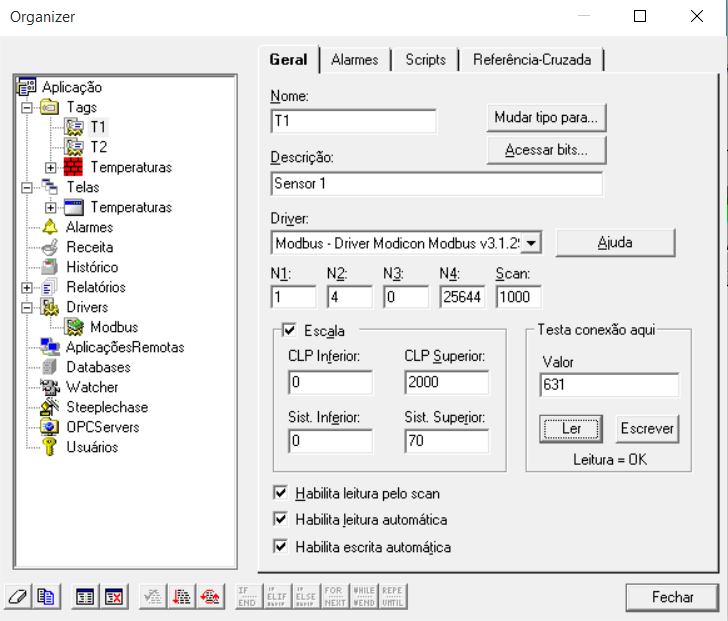
\includegraphics[scale=0.7]{Organizer.png}
\caption{\textit{Organizer} da aplicação}
\label{fig:Organizer}
\end{figure}

O valor definido na $Escala$ depende da resolução do sinal analógico gerado pelo CLP. No caso do TPW-03, utilizou-se o modo de entrada de corrente 4 - 20mA para conectar os sensores, o que nos dá uma resolução de 0 à 2000 unidades \cite{weg2010manualinstalacao}[p.65]. Dessa forma, configura-se a escala de 0 à 2000 unidades para o CLP indicando uma variação de temperatura proporcional de 0 a 70 ºC. Essa faixa de temperatura é estabelecida de acordo com os valores aos quais os transmissores dos sensores estão configurados.

A configuração do modo de operação do módulo 8AD é feita através da programação em Ladder no TPW03-PCLINK conforme explicado no item 3.2.1.


\section{Testes Desenvolvidos}

Feita a configuração de todos os parâmetros, associa-se as \textit{tags} a cada objeto criado através da própria tela da aplicação. Isso fará com que os objetos mostrem os valores lidos pelas \textit{tags} que representam as temperaturas dos sensores conectados aos controladores, logo, as medidas desejadas são mostradas nos elementos. Um exemplo da aplicação em atividade é observado na Figura \ref{fig:InterfaceRun}.

\begin{figure}[ht!]
\centering
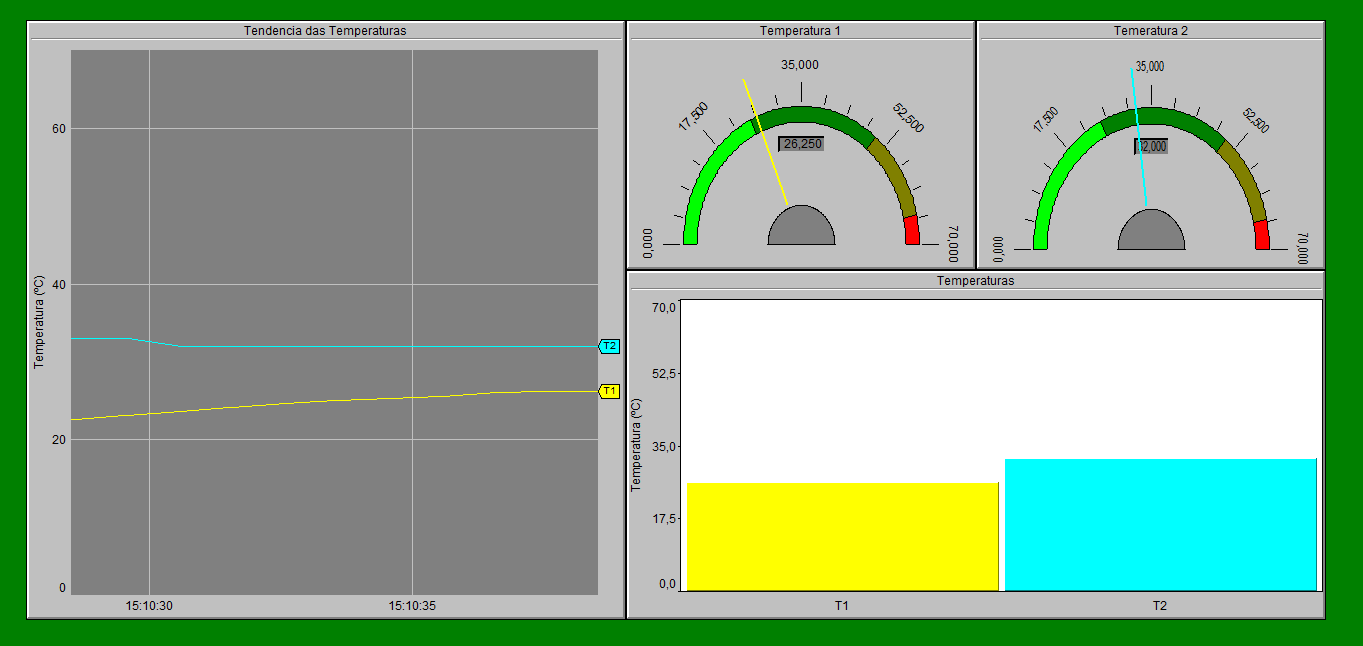
\includegraphics[scale=0.40]{InterfaceRun.png}
\caption{Aplicação em Execução}
\label{fig:InterfaceRun}
\end{figure}


Observa-se que os valores das temperaturas medidas nos dois sensores estão mostrados em todos os elementos da aplicação. Para testar o sistema, variou-se a temperatura nos dois sensores, conforme é observado no gráfico 'Tendência das Temperaturas'. O sensor que estava conectado ao TPW03 foi submetido à um aumento de temperatura simulado pelo contato dele a um corpo mais quente (temperatura de uma mão humana) enquanto o sensor conectado ao controlador N2000 foi submetido à uma diminuição de temperatura simulada por um copo de água gelada. As temperaturas obtidas durante o teste são coerentes, variando entre cerca de 20ºC e 35ºC.




%XXXXXXXXXXXXXXXXXXXXXXXXXXXXXXXXXXXXXXXXXXXXXXXXXXXXXXXXXXXXXXXXXXXXXXXXXXXXXXXXXXXXXXXXXXXXXXXXXXXXXXXX






\mychapter{Conclus\~{a}o}
\label{Cap:conclusao}



% Refer\^{e}ncias bibliogr\'{a}ficas (geradas automaticamente)

\addcontentsline{toc}{chapter}{Refer\^{e}ncias bibliogr\'{a}ficas}
\nocite{*}
\bibliography{bibliografia}


\appendix

% Ap\^{e}ndice A
%\include{apendice/apendice}

% Ap\^{e}ndice B
%\include{apendice/apendiceB}

% Ap\^{e}ndice C
%\include{apendice/apendiceC}

\end{document} 